\documentclass[12pt]{article}
\usepackage[utf8]{inputenc}
\usepackage{amsmath, amssymb, amsthm}
\usepackage{geometry}
\usepackage{tikz}
\usepackage{pgfplots}
\usepackage{tikz-3dplot}
\geometry{margin=1in}
\title{Glibert Strang's Linear Algebra}
\author{Jazmin Velez}
\date{\today}

\begin{document}

\maketitle

\title{Chapter 1: Matrices and Gaussian Elimination}

\section{Matrices and Gaussian Elimination}
\subsection{Introduction}
\begin{itemize}
    \item Two ways to solve a system of equations:
    \begin{enumerate}
        \item *Elimination - Gaussian elimination is consistently used to solve large systems of equations.
        \item Determinants
    \end{enumerate}
    \item Two ways in which elimination can break down:
    \begin{enumerate}
        \item If the system is inconsistent, it has no solutions.
        \item If the system is dependent, it has infinitely many solutions.
    \end{enumerate}
\end{itemize}

\subsection{The Geometry of Linear Equations}
\begin{itemize}
    \item A linear equation in two variables can be represented as a line in the plane.
    \item A linear equation in three variables can be represented as a plane in three-dimensional space.
    \item Two ways to visualize systems of linear equations:
    \begin{enumerate}
        \item \underline{Row form}: Each equation is represented as a line or plane in space, and the solution is the intersection of these lines or planes.
        \begin{align}
            2x &- y = 1\\
            x &+ y = 5
        \end{align}
        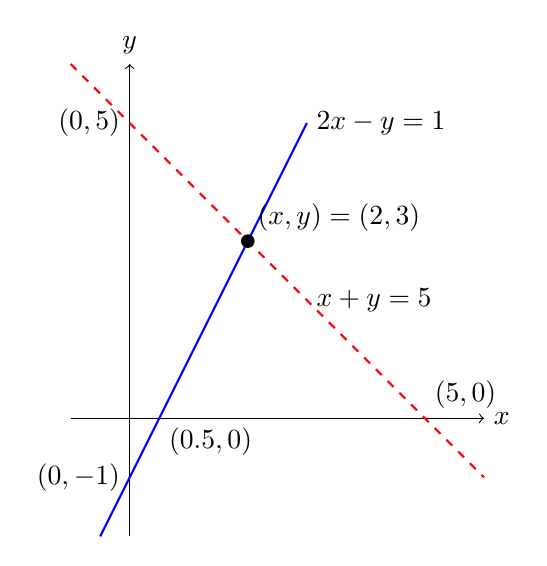
\begin{tikzpicture}[scale=0.75]
          % Axes
          \draw[->] (-1,0) -- (6,0) node[right] {$x$};
          \draw[->] (0,-2) -- (0,6) node[above] {$y$};

          % First line 2x-y=1; from (-1,-3) to (3,5)
          \draw[blue, thick] (-0.5,-2) -- (3,5);
          \node[right] at (3,5) {$2x - y = 1$};
          \node[left] at (0,-1) {$(0,-1)$};
          \node[below right] at (0.5,0) {$(0.5,0)$};

          % Second line x+y=5; from (-1,6) to (6,-1)
          \draw[red, thick, dashed] (-1,6) -- (6,-1);
          \node[right] at (3,2) {$x + y = 5$};
          \node[left] at (0,5) {$(0,5)$};
          \node[above right] at (5,0) {$(5,0)$};

          \filldraw[black] (2,3) circle (3pt) node[anchor=south west]{$(x, y) = (2,3)$};

        \end{tikzpicture}

        \item \underline{Column form}: Each variable is represented as a vector in space, and the solution is a linear combination of these vectors.
        \begin{align}
            x\begin{bmatrix}
                2\\
                1
            \end{bmatrix}
            + y\begin{bmatrix}
                -1\\
                1
            \end{bmatrix}
            =
            \begin{bmatrix}
                1 \\
                5
            \end{bmatrix}
        \end{align}
        \begin{tikzpicture}[scale=0.75]
          % Axes
          \draw[->] (-3.5,0) -- (4.5,0) node[right] {$x$};
          \draw[->] (0,-0.5) -- (0,5.5) node[above] {$y$};

          % First column vector [2, 1]
          \draw[blue, thick, ->] (0,0) -- (2,1);
          \node[below right] at (2,1) {$[2\,\,1]$};

          % Second column vector [-1, 1]
          \draw[red, thick, ->] (0,0) -- (-1,1);
          \node[below right] at (-1,1) {$[-1\,\,1]$};

          % First column vector * 2 = [4, 2]
          \draw[blue, thick, ->] (0,0) -- (4,2);
          \node[below right] at (4,2) {$2 * [2\,\,1] = [4\,\,2]$};

          % Second column vector [-1, 1] * 3 = [-3, 3]
          \draw[red, thick, ->] (0,0) -- (-3,3);
          \node[below left] at (-3,3) {$3 * [-1\,\,1] = [-3\,\,3]$};

          % Linear combination starting from 3 * second column vector
          \draw[blue, dashed, ->] (-3,3) -- (1,5);
          
          % Linear combination starting from 2 * first column vector
          \draw[red, dashed, ->] (4,2) -- (1,5);
         
          % Point at (2*first vector) + (3*second vector)
          \filldraw[black] (1,5) circle (3pt) node[anchor=south west]{$2[2\,\,1] + 3[-1\,\,1] = [1\,\,5]$};

        \end{tikzpicture}
    \end{enumerate}
    
    \item Example -- Visualizing Planes in 3D
        \begin{itemize}
            \item Row Form:
            \begin{alignat}{3}
                2u\ &{}+\ v\ &{}+\ w\ &=\ 5 \\
                4u\ &{}-\ 6v\ &\phantom{{}+ w} &=\ -2 \\
                -2u\ &{}+\ 7v\ &{}+\ 2w\ &=\ 9
            \end{alignat}
            \item Column Form:
            \begin{align}
                u\begin{bmatrix}
                    &2\\
                    &4\\
                    -&2
                \end{bmatrix}
                + v\begin{bmatrix}
                    &1\\
                    -&6\\
                    &7
                \end{bmatrix}
                + v\begin{bmatrix}
                    &1\\
                    &0\\
                    &2
                \end{bmatrix}
                =
                \begin{bmatrix}
                    &5\\
                    -&2\\
                    &9
                \end{bmatrix}
                = b
            \end{align}
            \item Matrix Representation$($simplifies notation$)$: \(\mathbf{A} \mathbf{x} = \mathbf{b}\)
            \begin{align}
                \mathbf{A} = \begin{bmatrix}
                    2 & 1 & 1 \\
                    4 & -6 & 0 \\
                    -2 & 7 & 2
                \end{bmatrix}, \quad
                \mathbf{x} = \begin{bmatrix}
                    u \\
                    v \\
                    w
                \end{bmatrix}, \quad
                \mathbf{b} = \begin{bmatrix}
                    5 \\
                    -2 \\
                    9
                \end{bmatrix}
            \end{align}
        \end{itemize}
    
    
%    \tdplotsetmaincoords{70}{110} % Adjust view angles
%    \begin{tikzpicture}[tdplot_main_coords, scale=1]
%        % Axes
%        \draw[->] (0,0,0) -- (5.5,0,0) node[anchor=north east]{$u$};
%        \draw[->] (0,0,0) -- (0,5.5,0) node[anchor=north west]{$v$};
%        \draw[->] (0,0,0) -- (0,0,5.5) node[anchor=south]{$w$};

%     $THIS GRAPH NEEDS TO BE FIXED!! The first plane is right-ish
%        % First Equation Plane
%        \fill[blue!30, opacity=0.6] (5/2,0,0) -- (0,5,0) -- (-5/2,5,5) -- (0,0,5) -- cycle;

%        % Second Equation Plane
%        \fill[red!30, opacity=0.6] (0,0,0) -- (0,3,0) -- (0,3,3) -- (0,0,3) -- cycle;

%        % Third Equation Plane
%        \fill[green!30, opacity=0.6] (0,0,0) -- (3,0,0) -- (3,0,3) -- (0,0,3) -- cycle;

%        % Labeled points
%        \filldraw[black] (2,2,2) circle (1pt) node[anchor=south west]{$(2,2,2)$};
%        \filldraw[black] (1,0,3) circle (1pt) node[anchor=north east]{$(1,0,3)$};
%        \filldraw[black] (0,2,1) circle (1pt) node[anchor=north west]{$(0,2,1)$};
%    \end{tikzpicture}

\end{itemize}
% Your content goes 

\end{document}